\section{Understanding Data via Interactive Visualisation}
\subsection{Network Data}


Networks are often the most convenient way to represent interactions among entities in social, biological, infrastructure and other information systems \cite{becker1995visualizing, herman2000graph}. 
Examples of network data include interactions among people in social networks, connectivity of web pages in world wide web graphs, and protein-protein interaction (PPI) in biological networks \cite{leskovec2014snap, arifuzzaman2017scalable}. 
Network analysis and visualization (also called Network Graph) help discover structures and patterns in a network and thereby reveal useful insights \cite{herman2000graph, arifuzzaman2015space, arifuzzaman2012patric, arifuzzaman2017scalable, arifuzzaman2015fast}.

Network data contains complex relationships between a huge amount of elements. A network visualization displays directed and undirected graph structures which illuminates relationships between entities. Elements or entities are usually displayed as round nodes and lines show the relationships between them. Network visualization is essential in multiple fields to simplify complex systems. For example, it is used in cyber security to better understand cyber threats, reveal network vulnerabilities, detect malware and discover trends. Moreover, in infrastructure management to create interactive visualization that reveal bottlenecks and vulnerabilities in connected critical infrastructure. And many other applications in social networks and biological networks. 


Some simple network data can be visualized simply using a static network visualization like the network visualization representing the metro stations in Figure~\ref{fig:metro}.

\begin{figure}[H]
\centering
\captionsetup{justification=centering}
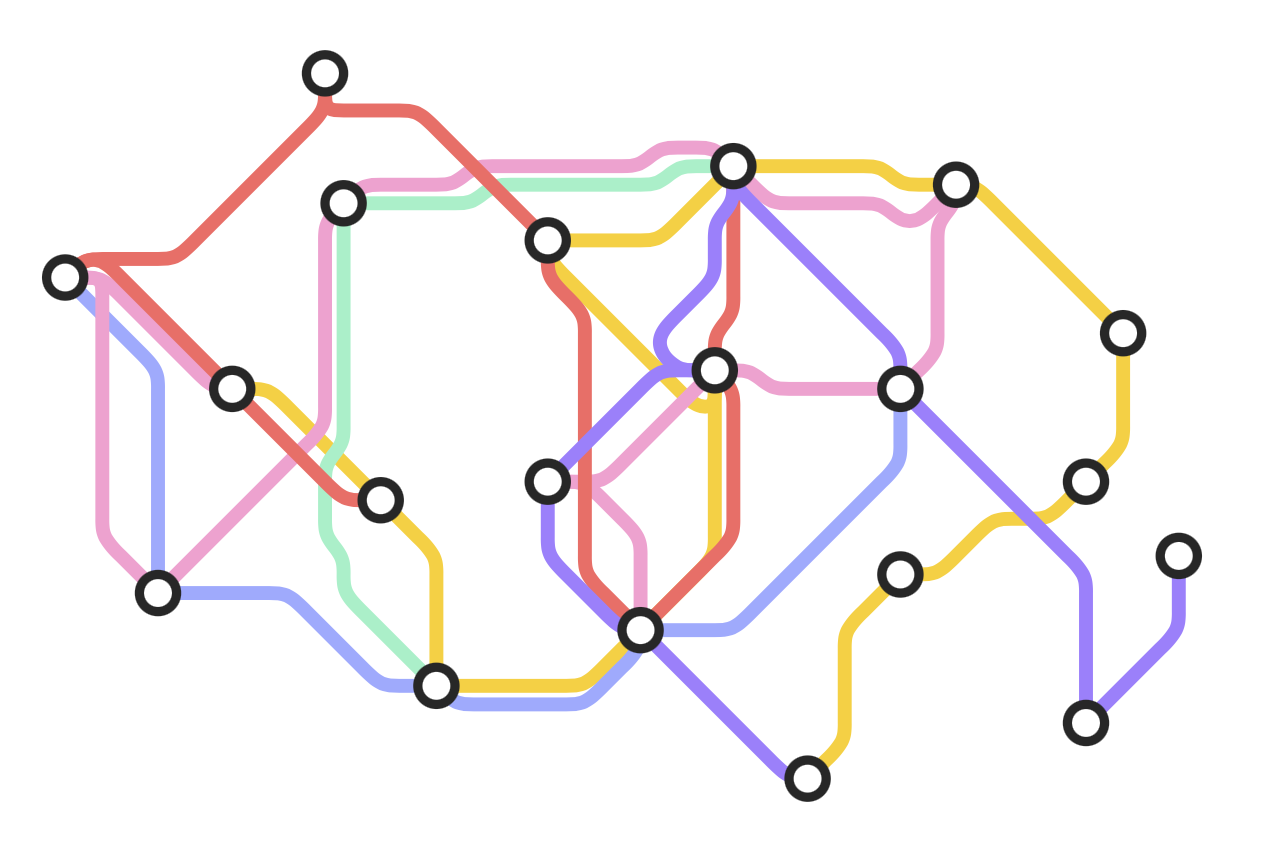
\includegraphics[width=0.9\textwidth]{./pics/network1.png}
\caption{Metro stations as network diagrams \cite{metro} }
\label{fig:metro}
\end{figure}

However most network data are big and complex containing multiple layers and many interactions which make it, if displayed naively, unreadable. 

\begin{figure}[H]
\begin{subfigure}{.45\textwidth}
  \centering
  \captionsetup{justification=centering}
  % include first image
  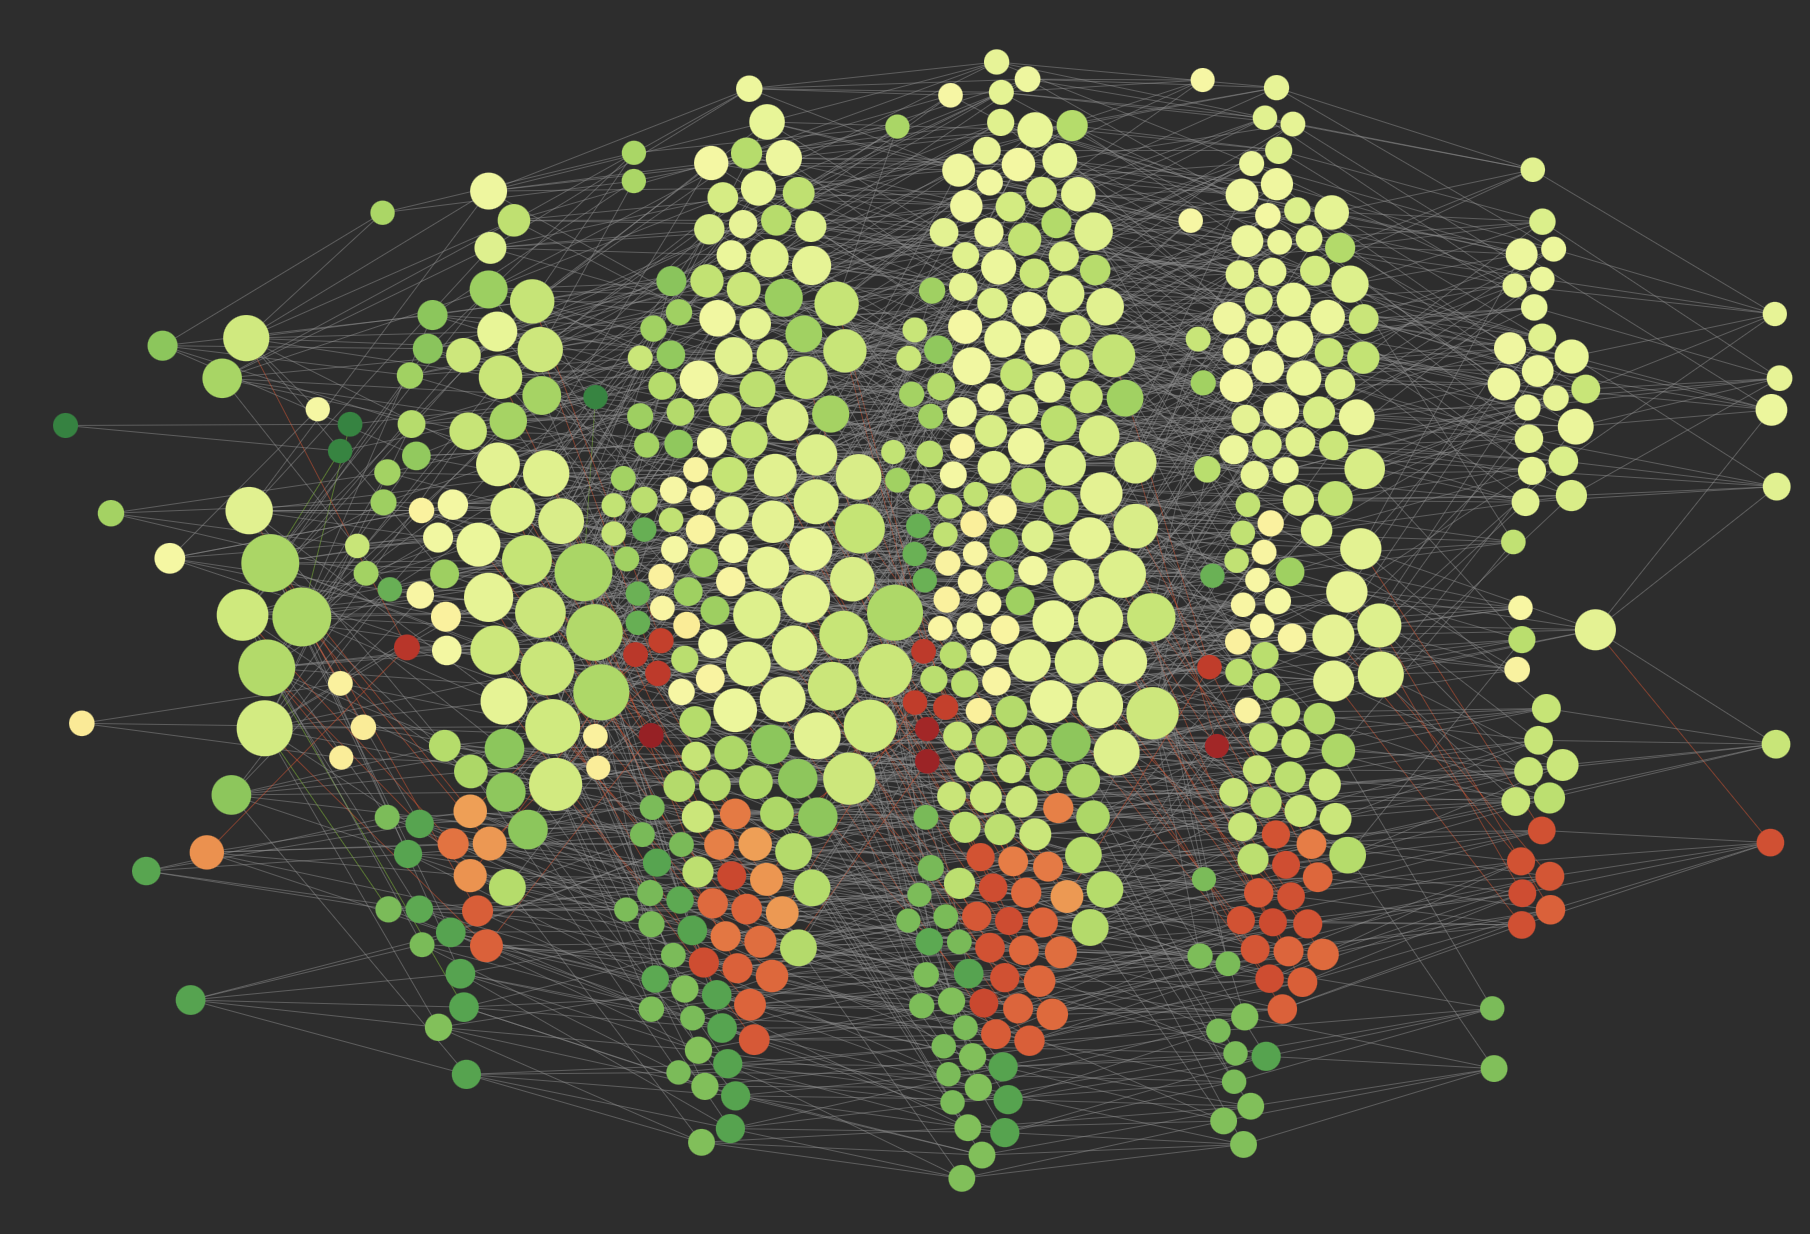
\includegraphics[width=.8\linewidth]{./pics/network21.png}  
  \caption{The whole network graph}
  \label{fig:sub-first-network}
\end{subfigure}
\begin{subfigure}{.45\textwidth}
  \centering
  \captionsetup{justification=centering}
  % include second image
  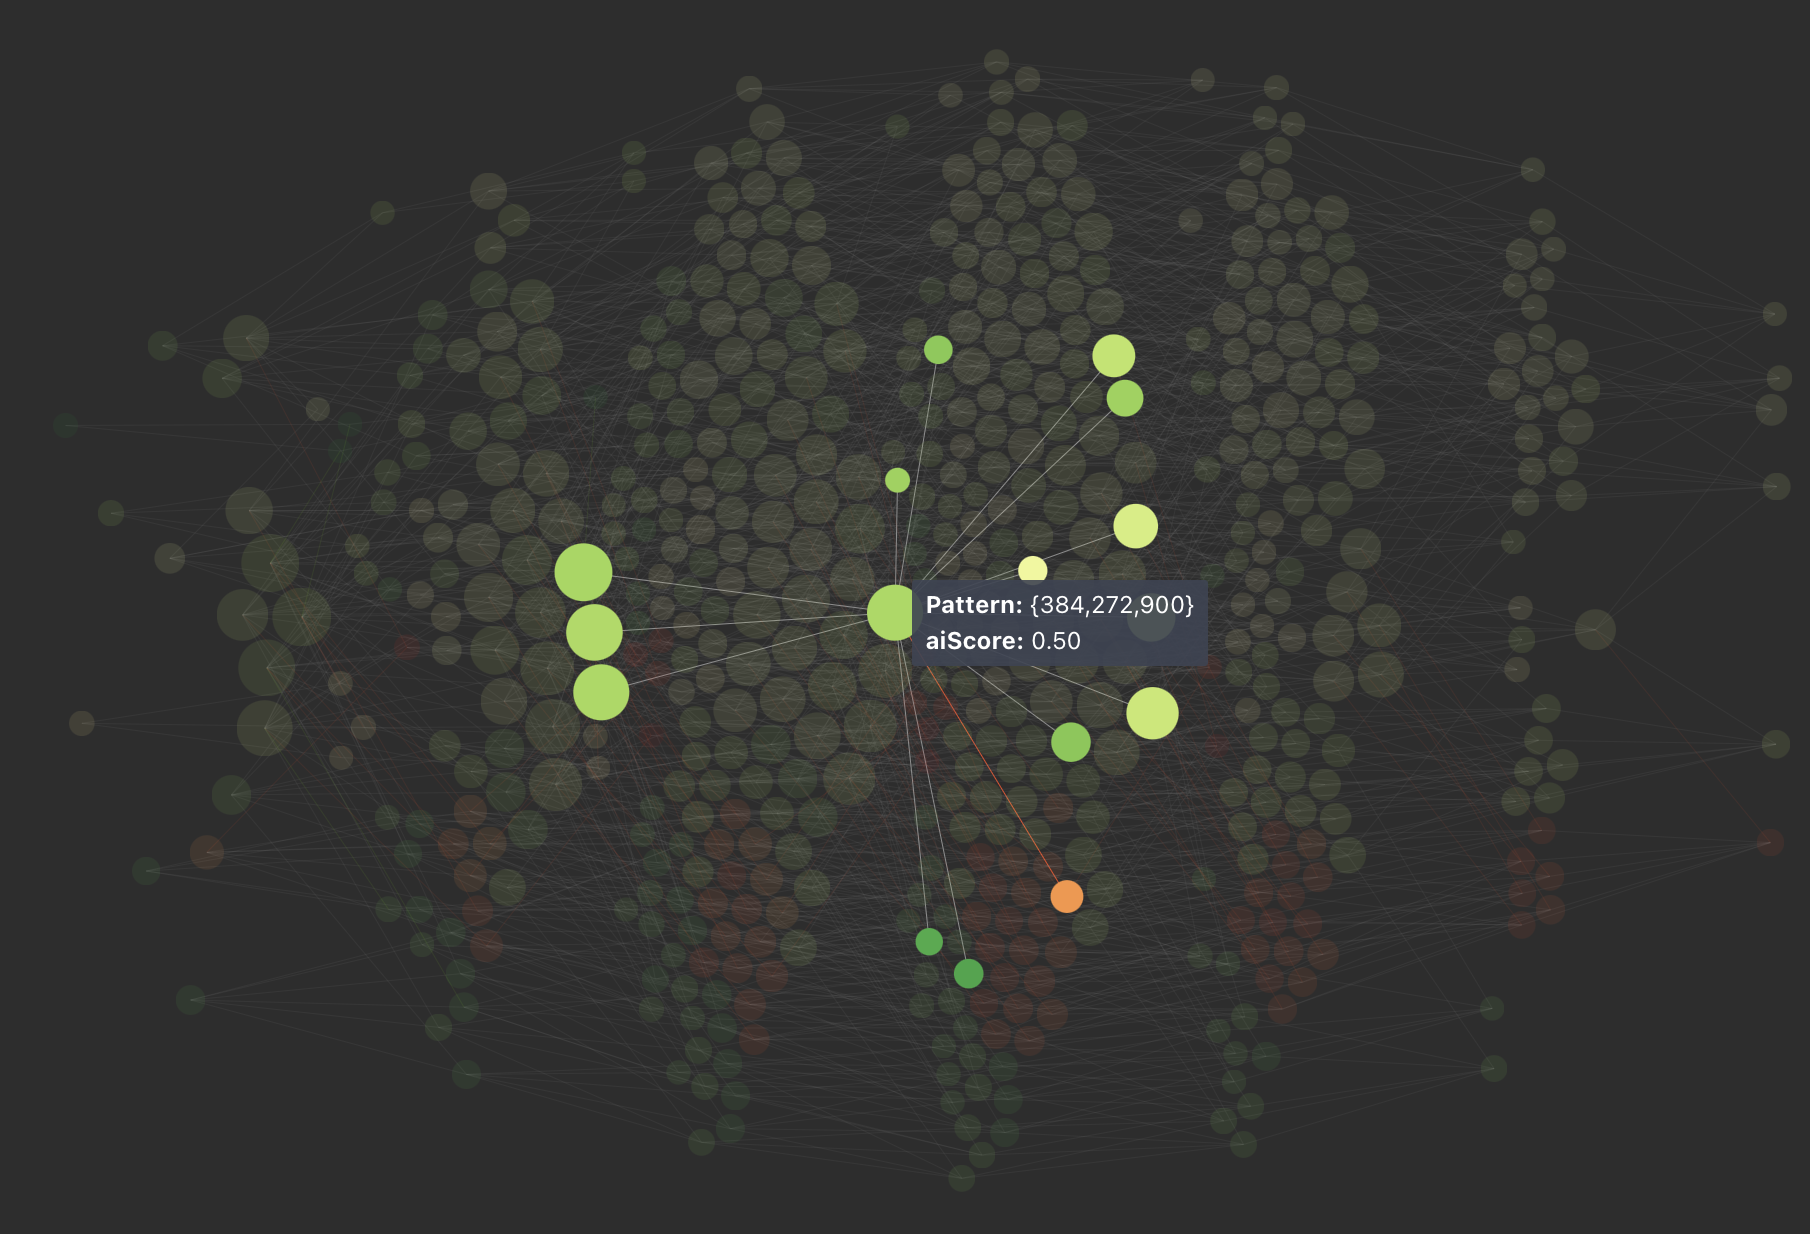
\includegraphics[width=0.8\linewidth]{./pics/network22.png}  
  \caption{Focus on just one pattern}
  \label{fig:sub-second-focus-network}
\end{subfigure}
\captionsetup{justification=centering}
\caption{Network of pattern in medical compound dataset \cite{networkgraph}}
\label{fig:network-graph}
\end{figure}

\subsection{Causal Inference}

Not statistical but causal questions motivate most quantitative studies in the health, social and behavioral sciences \cite{pearl2011science}. Causality is always a tricky subject and it is often mixed with correlation. A correlation is when two variables tend to change together and it does not necessarily indicate causation. For example Figure~\ref{fig:temp} from the BBC news, shows that the number of crimes in London rises with temperature. This can easily mislead the viewers to conclude that warmer temperature causes violent crimes \cite{matute2015illusions}.

\begin{figure}[H]
\centering
\captionsetup{justification=centering}
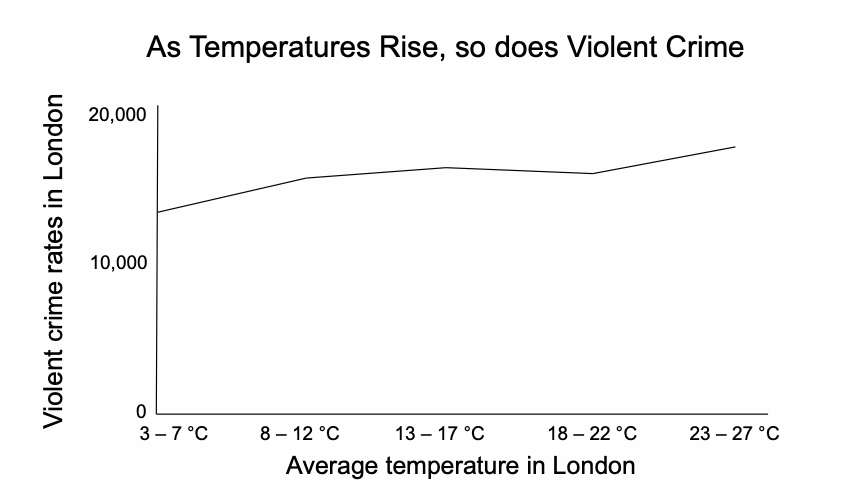
\includegraphics[width=0.9\textwidth]{./pics/casual1.png}
\caption{Recreation of BBC news article figure, ``Heatwave: Is there more crime in hot weather?"\cite{matute2015illusions} }
\label{fig:temp}
\end{figure}


It is difficult to distinguish causation from correlation \cite{rothman2012epidemiology}. Only a correlation was established between temperature and crime rate in this case because it is likely that there are other factors not shown in this static graph that could influence the number of violent crimes in both cases. Even journalists and researchers can amplify causal implications from such results which in many cases mislead the audience. 

As causality is hard to be identified so a static visualization is confusing since it can only show just one to a few factors while there might be many other factors to analyze to reveal hidden insights. 

Interactive visualization could help by providing filtering or multiple strategies with all factors presented to help look at all the possible variables together or by customizing the view and look at them in many different ways to facilitate the process and strengthen the judgments. 

\begin{figure}[H]
\centering
\captionsetup{justification=centering}
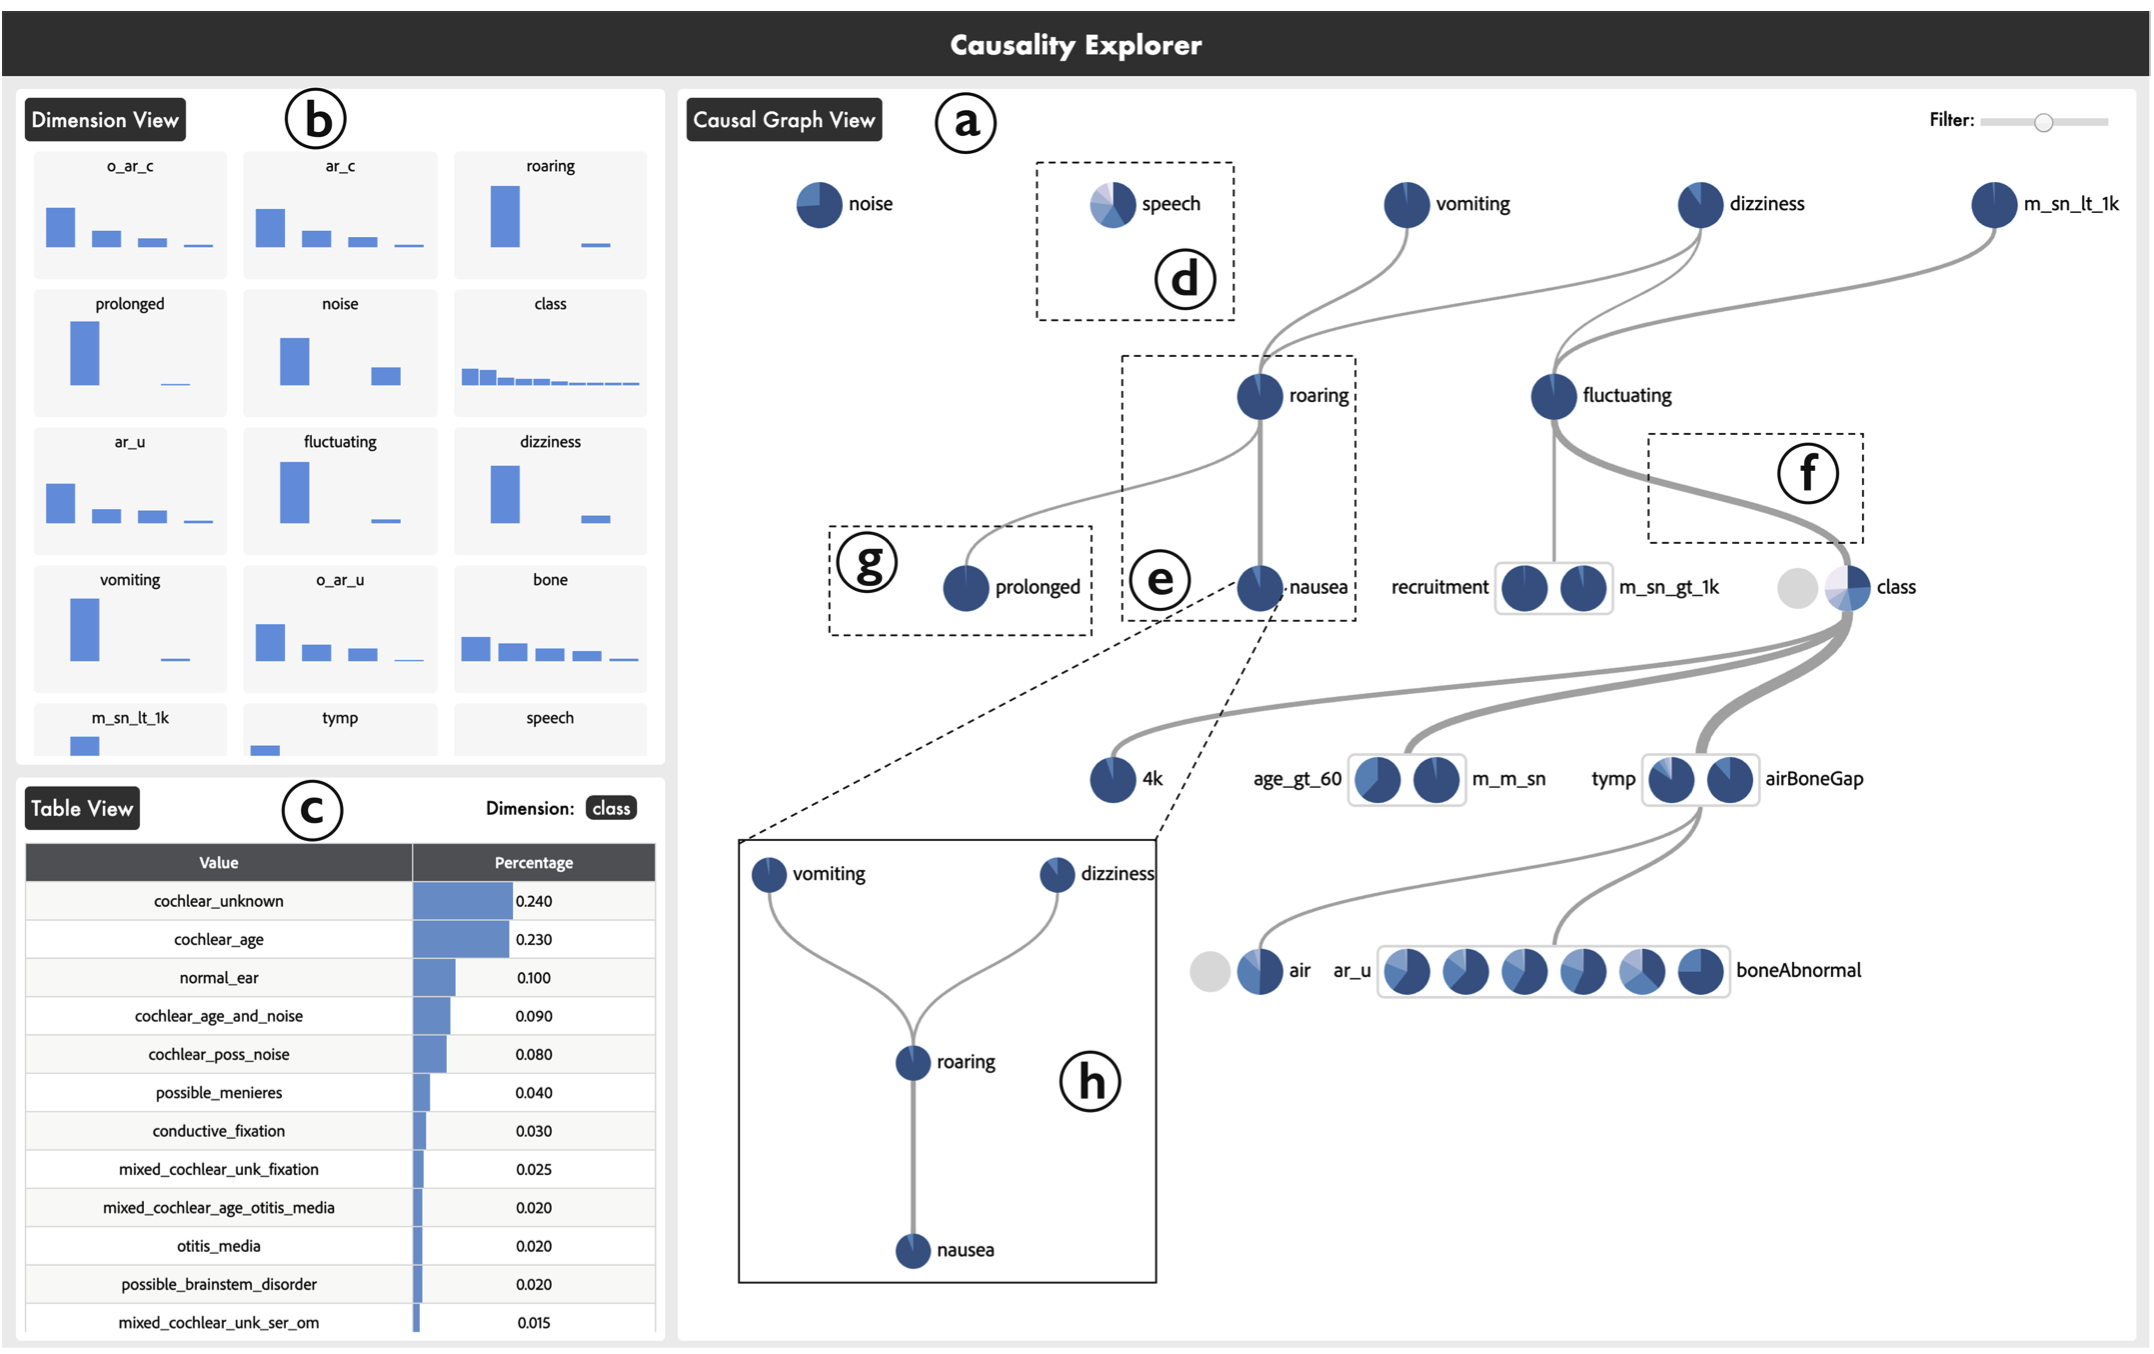
\includegraphics[width=0.9\textwidth]{./pics/cas.png}
\caption{The interactive user interface of Causality Explorer\cite{dua2017uci}. (a) is the interactive scalable causal graph and (b) \& (c) are views for comparative analysis to support what-if analyses.}
\label{fig:cas}
\end{figure}



\subsection{Time Series Data}

The line graph is the simplest and the most common way to represent time series data. It does help the viewer to observe what has changed over time. Statistically visualizing one or few variables in a small to medium dataset is very useful and has many applications and it is one of the most common visualization type in media. The problem rises when there is a big dataset and tens to hundreds variables to be displayed over a time-period. It is not possible to visualize a hundred attributes over a time-period in just one statistic visualization nor having a hundred separate visualization for each attribute which will be overwhelming and impossible to conclude any useful insights or correlations. For example, as shown in Figure~\ref{fig:loaded-lines}, it is confusing and overwhelming to look at the data and come out with useful insights.

\begin{figure}[H]
\centering
\captionsetup{justification=centering}
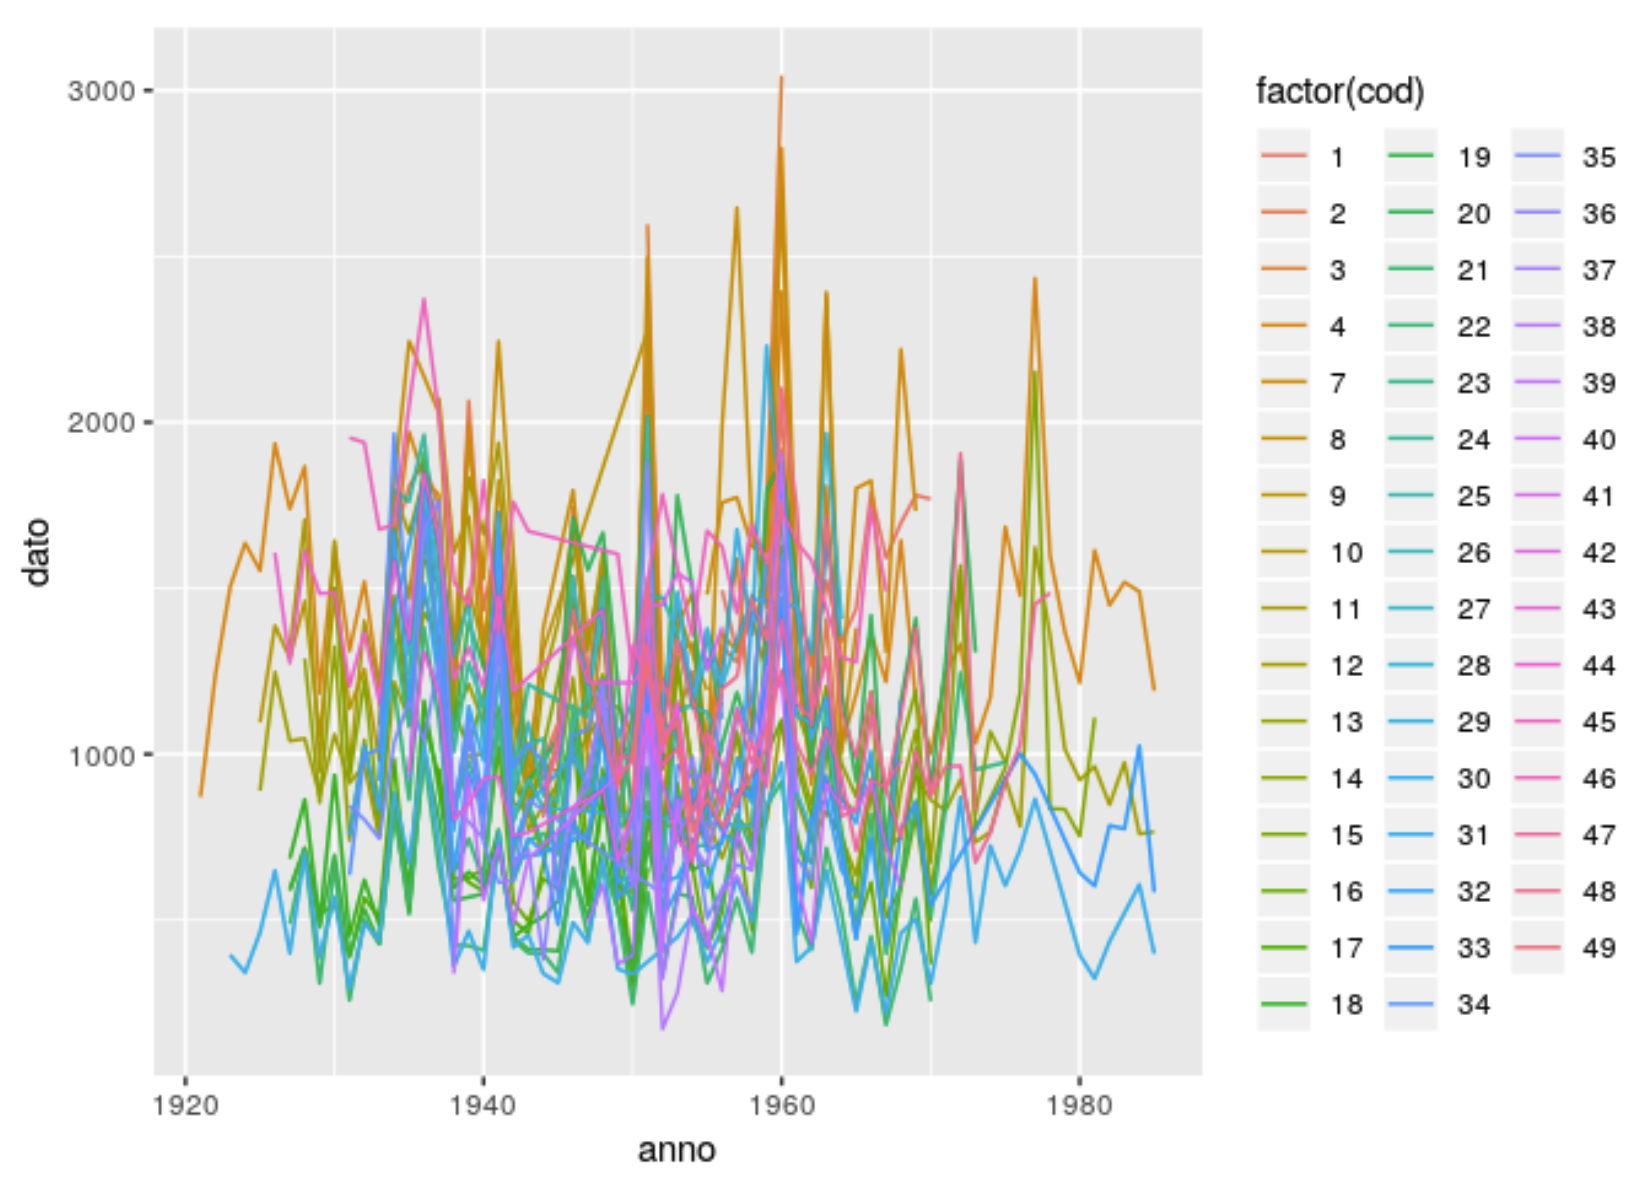
\includegraphics[width=0.9\textwidth]{./pics/loadedl.png}
\caption{Example of a loaded time series data Visualization \cite{loadedtimeseries}}
\label{fig:loaded-lines}
\end{figure}

Moreover, a static time-series visualization over a long period can eliminate the details and only show the full picture.
Interactive visualization offers the customization and the freedom to explore and customize the visualization to the user's needs. It gives the user the ability to have many different static visualizations in just one display. In Figure~\ref{fig:interactive-ts}, Only the focus strategy was introduced to the graph and it made a huge difference by almost eliminating all other attributes. 

\begin{figure}[H]
\begin{subfigure}{.45\textwidth}
  \centering
  \captionsetup{justification=centering}
  % include first image
  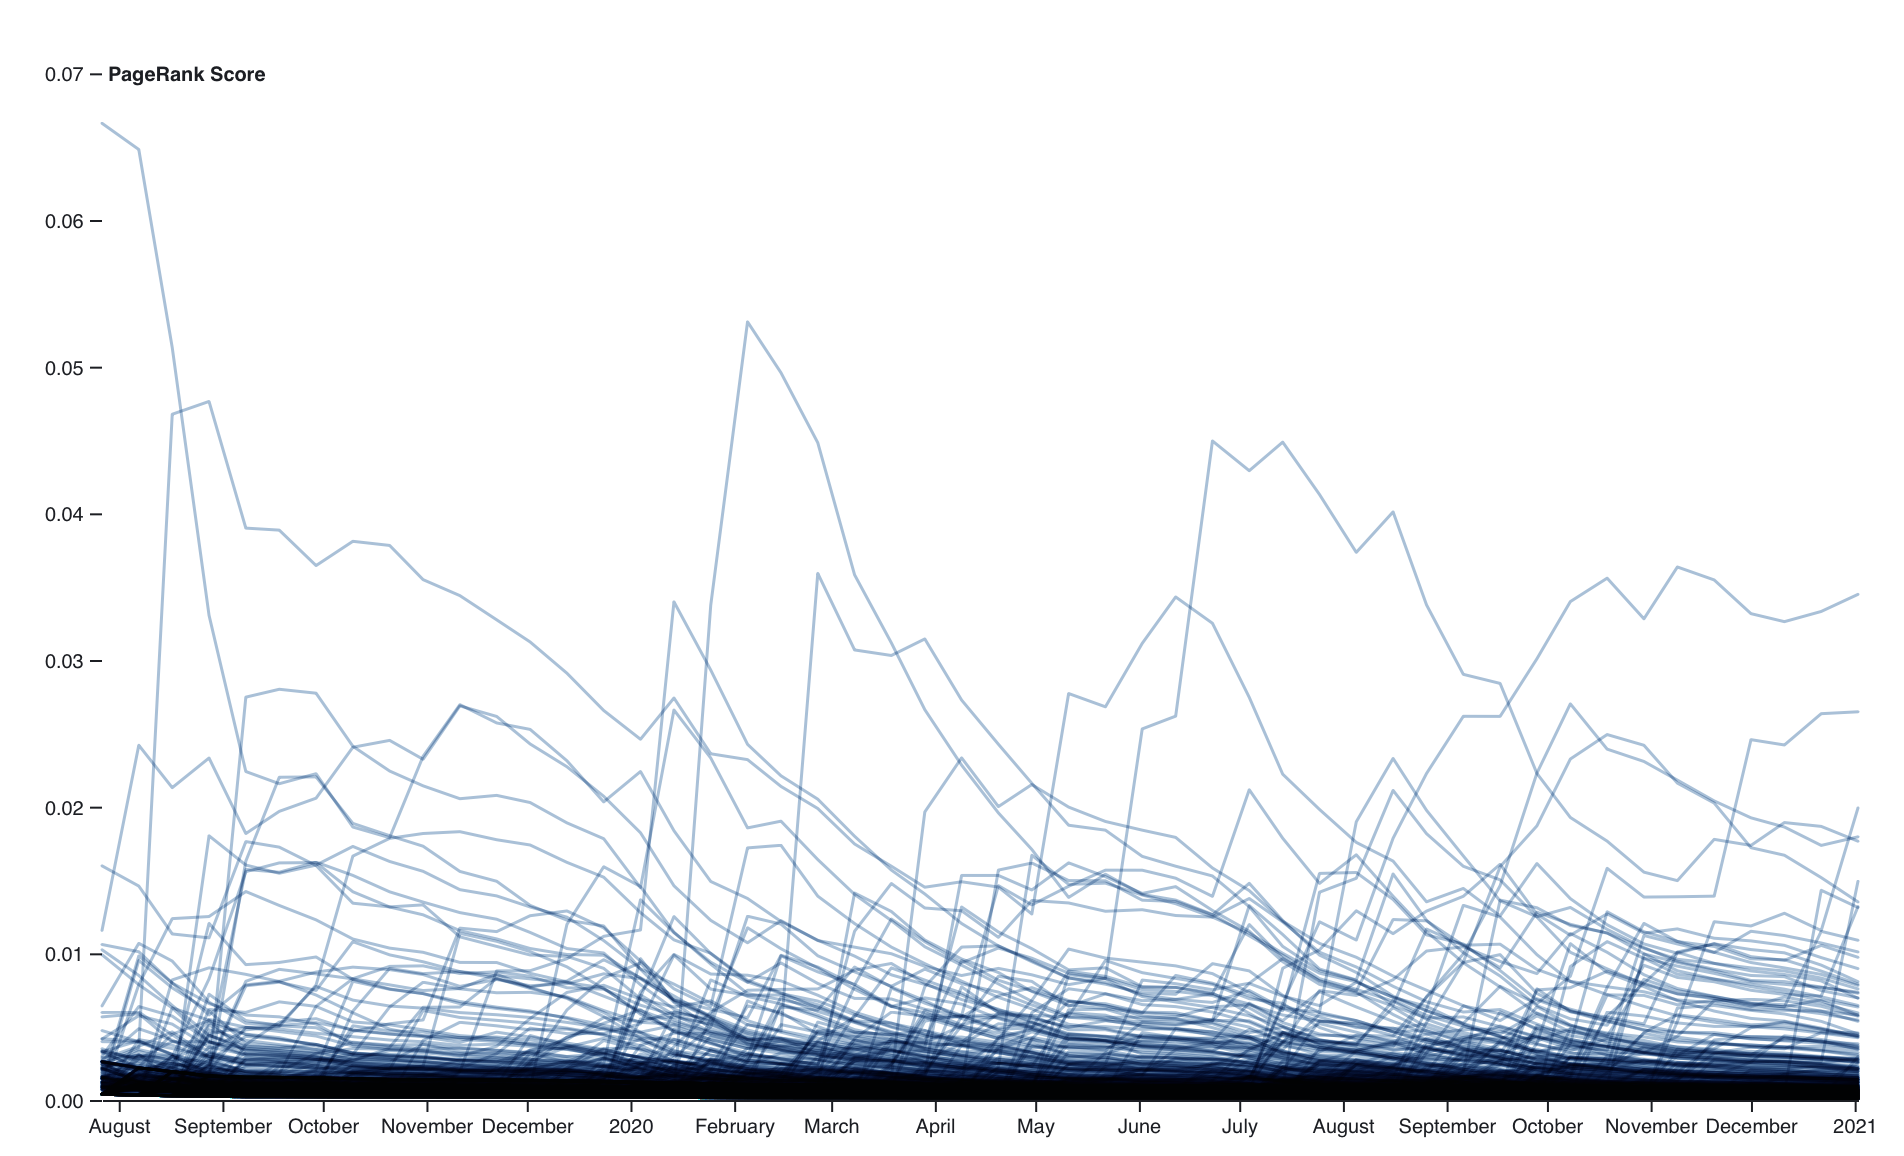
\includegraphics[width=.8\linewidth]{./pics/time21.png}  
  \caption{The whole time series data graph}
  \label{fig:sub-first-time21}
\end{subfigure}
\begin{subfigure}{.45\textwidth}
  \centering
  \captionsetup{justification=centering}
  % include second image
  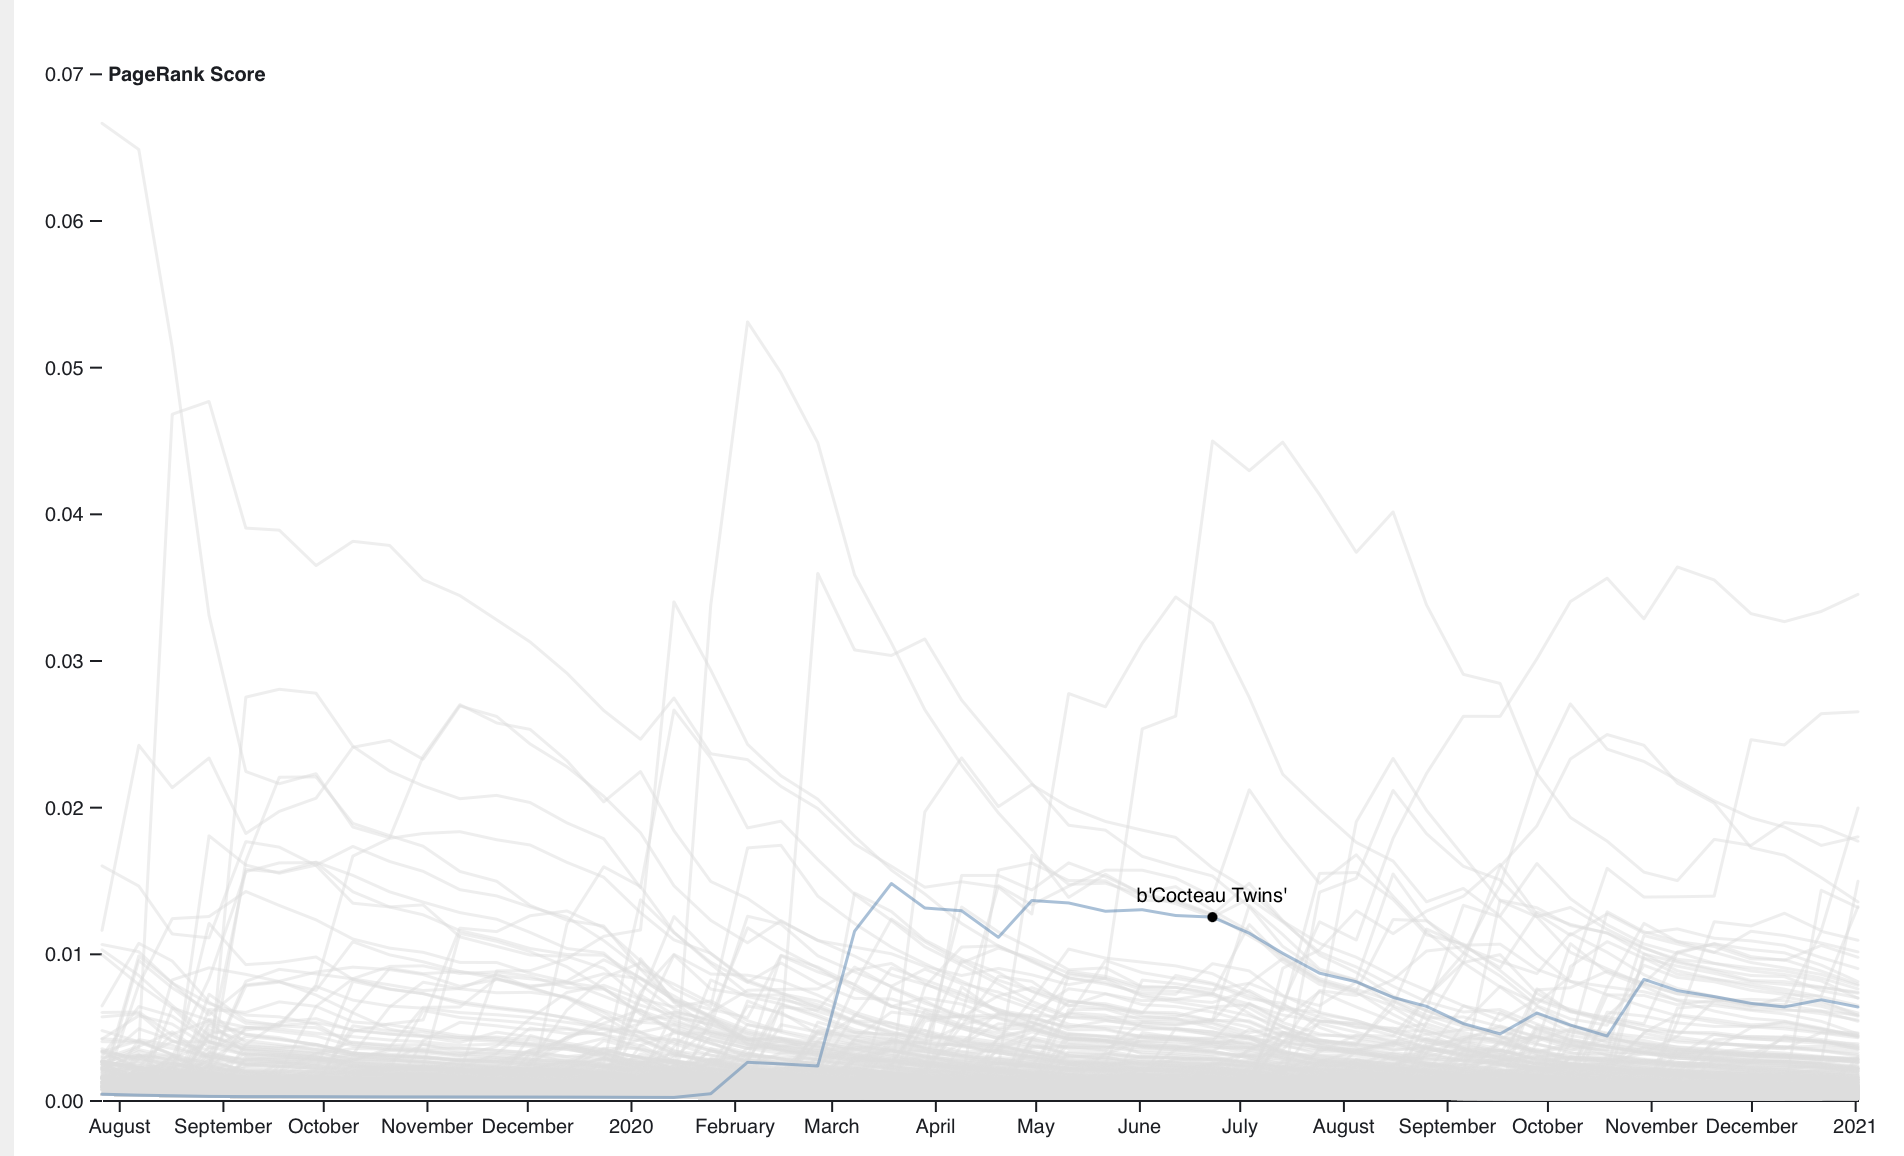
\includegraphics[width=0.8\linewidth]{./pics/time22.png}  
  \caption{Focus on just one attribute}
  \label{fig:sub-second-time22}
\end{subfigure}
\captionsetup{justification=centering}
\caption{Interactive time series data Visualization with focus strategy \cite{multiplelines} }
\label{fig:interactive-ts}
\end{figure}

% \\\  You cannot do this in TeX! RAAZ 

In another example like the one shown in Figure~\ref{fig:interactive-focus-filter}, both filter and focus strategies were used which gives the user all the possible ways to view the time series data. In other cases, the zoom strategy could help in a long time series graph to zoom in to a short period and examine the data. 

\begin{figure}[H]
\centering
\captionsetup{justification=centering}
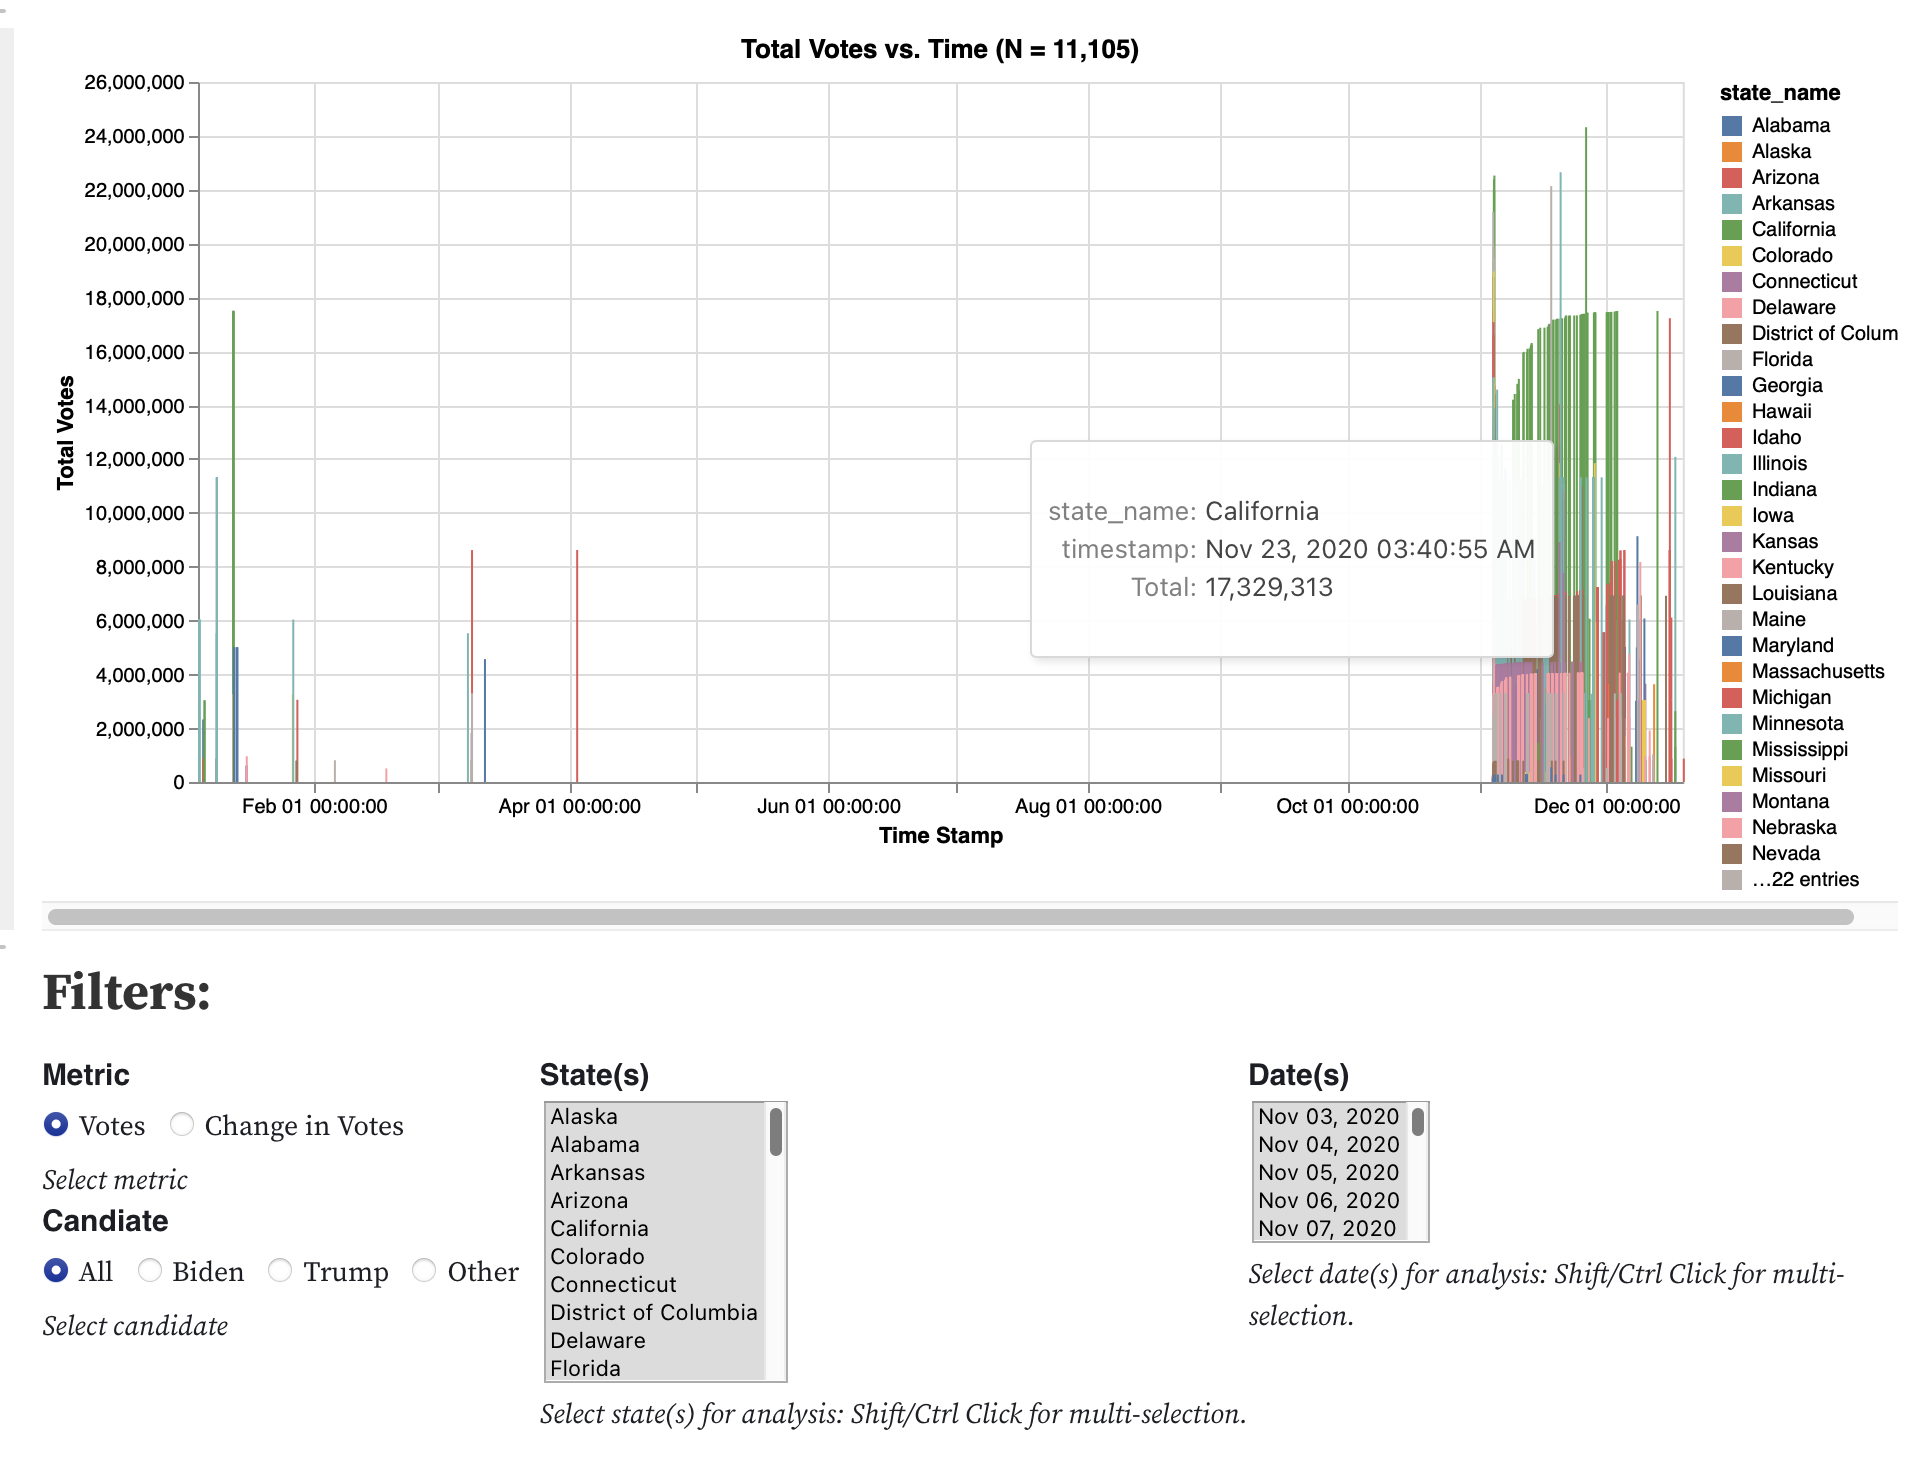
\includegraphics[width=0.9\textwidth]{./pics/time1.png}
\caption{Interactive time series data visualization with focus \& filter strategies \cite{2020timeseries} }
\label{fig:interactive-focus-filter}
\end{figure}
